\documentclass[a4paper,12pt]{article}

%%% Работа с русским языком
\usepackage{cmap}					% поиск в PDF
\usepackage{mathtext} 				% русские буквы в формулах
\usepackage[T2A]{fontenc}			% кодировка
\usepackage[utf8]{inputenc}			% кодировка исходного текста
\usepackage[english,russian]{babel}	% локализация и переносы
\usepackage{indentfirst}
\frenchspacing

%%% Страница
\usepackage{extsizes} % Возможность сделать 14-й шрифт
\usepackage{geometry} % Простой способ задавать поля
\geometry{top=20mm}
\geometry{bottom=20mm}
\geometry{left=30mm}
\geometry{right=15mm}

\usepackage{hyperref}

\RequirePackage{color,graphicx, colortbl}
\graphicspath{{img/}}  

\usepackage[usenames,dvipsnames]{xcolor}
\usepackage[big]{layaureo} 				%better formatting of the A4 page
% an alternative to Layaureo can be ** \usepackage{fullpage} **
\usepackage{titlesec}					%custom \section

%Setup hyperref package, and colours for links
\usepackage{hyperref}
\definecolor{linkcolour}{rgb}{0,0.2,0.6}
\hypersetup{colorlinks,breaklinks,urlcolor=linkcolour, linkcolor=linkcolour}

%CV Sections inspired by: 
%http://stefano.italians.nl/archives/26
\titleformat{\section}{\Large\scshape\raggedright}{}{0em}{}[\titlerule]
\titleformat{\subsection}{\large\scshape\raggedright}{}{1cm}{}[\titlerule]
\titlespacing{\section}{0pt}{0.5cm}{3pt}
\titlespacing{\subsection}{1cm}{3pt}{3pt}
%Tweak a bit the top margin
%\addtolength{\voffset}{-1.3cm}
\usepackage[absolute]{textpos}

\setlength{\TPHorizModule}{30mm}
\setlength{\TPVertModule}{\TPHorizModule}
\textblockorigin{2mm}{0.65\paperheight}

\usepackage{tikz}
\usetikzlibrary{mindmap,shadows}
\usepackage{smartdiagram}
\smartdiagramset{
	bubble center node font = \footnotesize,
	bubble node font = \footnotesize,
	% specifies the minimum size of the bubble center node
	bubble center node size = 0.5cm,
	%  specifies the minimum size of the bubbles
	bubble node size = 0.5cm,
	% specifies which is the distance among the bubble center node and the other bubbles
	distance center/other bubbles = 0.3cm,
	% sets the distance from the text to the border of the bubble center node
	distance text center bubble = 0.5cm,
	% sets the opacity at which the bubbles are shown
	bubble fill opacity = 0.6,
	% sets the opacity at which the bubble text is shown
	bubble text opacity = 0.5,
}
\usepackage{multicol}
\usepackage{fontawesome}
\pdfmapfile{fontawesome.map}
\usepackage{multirow}
\usepackage{makecell}
\usepackage{longtable}
\usepackage{enumitem}

\pagenumbering{gobble}

\definecolor{linkedin}{HTML}{0085AE}
\definecolor{skype}{HTML}{12A5F4}
\definecolor{gmail}{HTML}{c71610}
\definecolor{kaggle}{HTML}{20beff}

\newcommand{\github}{ArtyomKaltovich}
\newcommand{\mail}{kaltovichartyom@gmail.com}
\newcommand{\skype}{artyomkaltovich}
\newcommand{\linkedin}{artyomkaltovich}

\newcommand{\WorkExpCompany}[2]{
    \multicolumn{2}{c}{\bfseries\emph{#1}}  & \bfseries #2 \\*
    \multicolumn{3}{c}{} \\*
}
\newcommand{\WorkExpProject}[5]{
        \multirow{4}{*}{} 
        & \em \makecell[r]{#1\\#2}  & #3 \\* 
        &Responsibilities & \small #4\\*
        &Environment & \small #5\\*
        \multicolumn{3}{c}{} \\
}

\begin{document}

\par{\centering{
		\Huge Artsiom \textsc{Kaltovich} \\ 
		\large Software Engineer\\
   		\large Minsk, Belarus
	}\bigskip
\par}

\begin{tabular}[\textwidth]{ll}
    \multirow{6}{*}{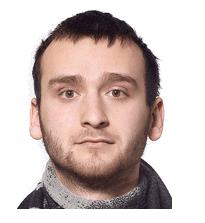
\includegraphics[width=4cm]{Artsiom_Kaltovich.jpg}\hspace{15mm}}   
    & \small links are clickable, but not in github preview :)\\
   	& \large\textnormal{\faGithub} {\href{https://github.com/\github}{\github}} \vspace{2mm} \\
    & \large\textnormal{\textcolor{kaggle}{\textbf{k}}} {\href{https://www.kaggle.com/linearleopard}{linearleopard}} \vspace{2mm} \\
   	& \large\textnormal{\textcolor{linkedin}{\faLinkedin}} \href{https://www.linkedin.com/in/\linkedin}{\linkedin} \vspace{2mm} \\
   	& \large\textnormal{\textcolor{gmail}{\faAt}} \href{mailto:\mail}{\mail} \vspace{2mm} \\
   	& \large\textnormal{\textcolor{skype}{\faSkype}} \href{skype:\skype?userinfo}{\skype} \vspace{2mm} \\ 
    & \vspace{2mm} \\
\end{tabular}

\section{Skills}

\begin{tabular}[\textwidth]{rl}
\smartdiagram[bubble diagram]{
    \textbf{Programming},
    \textbf{Python},
    \textbf{Java},
    \textbf{Asm},
    \textbf{html}\\\textbf{css},
    \textbf{xml},
    \textbf{sql}
} \hspace{10mm} &
\smartdiagramset{
	bubble center node size = 3.5cm,
}
\smartdiagram[bubble diagram]{
    \textbf{Personal},
    \textbf{Problem}\\\textbf{solver}, 
    \textbf{Respon}\\\textbf{sible},
    \textbf{Innova}\\\textbf{tive},
    \textbf{Ambitious},
    \textbf{funny}
} 
\end{tabular}

\subsection{Detail}
\hspace{0.75cm}
\begin{tabular}{lp{10cm}}
    Programming Languages:& \small Assembler (x86, z/OS, BS2000 OSD), C,C++, C\#, Cobol, Delphi, \textbf{Groovy}, \textbf{Java}, PHP, \textbf{Python}, SPL, \textbf{SQL}, Ruby \\ 
    Web Technologies:&\small .NET, J2EE, \textbf{Django}, Flask, Ruby on Rails\\ 
    Databases:&\small MS SQL, \textbf{MySQL}, SQLite, UDS/SQL\\ 
    Operating Systems:&\small Android, BS2000 OSD, \textbf{Linux}, Windows, z/OS\\ 
    Other Skills:&\small CSS, Eclipse SDK and RCP, IDEF, JFace, \textbf{git}, \LaTeX, \textbf{HTML}, Mathematica, Octave(Matlab), SWT, UML, \textbf{XML}, VHDL\\ 
\end{tabular} 

\subsection{Languages}
\hspace{0.75cm}
\begin{tabular}{rl}
    Belarussian: & Bilingual\\
    Russian: & Bilingual\\
    English: & Fluent\\
    German: & Intermediate\\
\end{tabular}
\newpage

\section{Work Experience}

\begin{longtable}{lr|p{11cm}}
    % SK Hynix
    \WorkExpCompany{Jun 2018 - present}{SK Hynix Memory Solutions Eastern Europe}
    \WorkExpProject{Jun 2018 - present}
        {\makecell[r]{Software Engineer}}
        {NAND Testing and Emulating}
        {Creating model and software for emulating and testing NAND Firmware}
        {Python, C}
        
    % Workfusion
    \WorkExpCompany{Dec 2017 – Jun 2018}{Workfusion}
    \WorkExpProject{Dec 2017 – Jun 2018}
        {\makecell[r]{Software Engineer}}
        {Automation Academy}
        {Providing environment for education of partners' students, included creating samples, Q\&A sessions, course creating and training, grading assignments, troubleshooting. Communication with development team on issues, future requests, implementation, etc}
        {Java, Selemium, XML, Web-Harvest, WorkFusion}
        
    % r to python
    \WorkExpCompany{Feb 2017 – Mar 2017}{Remote work/side project}
    \WorkExpProject{Feb 2017 – Mar 2017}
        {\makecell[r]{Data Sciencer\\Python Developer}}
        {Migrating pipeline of analyzing scientific data in bioinformatics research from R to Python}
        {Visualizing data, p-value, correlation and other metrics calculation}
        {Linux, Python, R, Matplotlib, Biopython, Bokeh, PyPlot, sklearn, pandas, Microsoft Excel, Libreoffice Calc}
    
    % IBA
    \WorkExpCompany{Jun 2013 – Dec 2017}{IBA Group}
    
    % astelit
    \WorkExpProject{Jul 2015 – Mar 2017}
        {Java Developer}
        {Astelit}
        {Upgrading ERP-system from IBM Maximo 5 to Maximo 7. Developing extension for Eclipse IDE. Migration applications workflows, user interfaces, database schema, custom PHP-reports. Designing and developing a solution to control, modify and remotely update resources, customizable local resources hierarchy and multiple Maximo 7 instances.}
        {Linux, Java, WebSphere, JSP, XML, SQL, PHP, Perl}
    
    %UDS
    \WorkExpProject{Jul 2013 – Dec 2017}
        {System Programmer}
        {BS2000 Tools: UDS/SQL}
        {Support and maintenance of UDS/SQL, including bug fixing, new features development, testing, new release/version creating}
        {BS2000, AID, COBOL, LMS, SDF, OpenFT, Assembler, SPL}
\end{longtable}

%Section: Education
\section{Education}
\begin{tabular}[\textwidth]{r|p{11cm}}
    % bsuir 
    \em Sep 2010 - Jun 2015  & \textbf{Belarusian State University of Informatics and Radioelectronics}, \textit{Minsk} \\
    Faculty & Computer System and Networks\\ 
    Department & Software for Information Technologies\\
    Thesis & Asynchronous encryption\\
    Average Mark & 8.8 \\
    \multicolumn{2}{c}{} \\	
\end{tabular}

\section{Scholarships and Certificates}
\begin{tabular}[\textwidth]{r|p{13cm}}
    \em Coursera
    & \textit{Machine Learning}~-~Stanford University\\
    & \textit{Cryptography I}~-~Stanford University\\
    & \textit{Introduction to Mathematical Thinking}~-~Stanford University\\
    & \textit{Biology Meets Programming: Bioinformatics for Beginners}~-~University of California San Diego\\
    & \textit{\textcyrillic{Теория игр} (Game Theory)}~-~National Research University Higher School of Economics (HSE), Moscow\\
    & \textit{Экономика для неэкономистов (Economics for non-economists)}~-~HSE, Moscow\\
    & \textit{Документы и презентации в LaTeX (Introduction to LaTeX)}~-~HSE, Moscow\\ 
    & \textit{Введение в машинное обучение (Introduction to Machine Learning)}~-~HSE, Moscow. Yandex School of Data Analysis (SDA)\\
    & \textit{Basic Modeling for Discrete Optimization}~-~The University of Melbourne, The Chinese University of Hong Kong\\
    \multicolumn{2}{c}{} \\	
    
    \em openedu.ru
    & \textit{Макроэкономика(Macroeconomics)} - HSE, Moscow\\
    & \textit{Анализ данных на практике (Data Analisys in Practice)} - Moscow Institute of Physics and Technology (MIPT)\\
    \multicolumn{2}{c}{} \\	
        
    \em stepik.org
    & \textit{\textcyrillic{Основы статистики} (Statistics: Basics)} - Computer Science Center (CSC - JetBrains, St.Petersburg)\\
    & \textit{\textcyrillic{Алгоритмы: теория и практика. Методы} (Algorithms: theory and practise. Methods)} - 
    Bioinformatics Institute, St.Petersburg\\
    & \textit{\textcyrillic{Алгоритмы: теория и практика. Структуры данных} (Algorithms: theory and practise. Data structures)} - 
    Bioinformatics Institute, St.Petersburg\\
    & \textit{\textcyrillic{Молекулярная биология и генетика} (Molecular Biology and Genetics)} - Bioinformatics Institute, St.Petersburg\\
    & \textit{\textcyrillic{Основы дискретной математики} (Discrete mathematics: Basics)} - Computer Science Center (CSC - JetBrains, St.Petersburg)\\
    & \textit{\textcyrillic{Математический анализ (часть 1)} (Calculus ()Part I))} - Computer Science Center (CSC - JetBrains, St.Petersburg)\\
    \multicolumn{2}{c}{} \\	
    
    \em udacity.com
    & \textit{ud120: Intro to Machine Learning}\\
\end{tabular}

\section{Interests and Activities}

Programming, Mathematics, Physics, History, Languages, Economy, Politics.\\
Dancing, Cooking, Traveling.

\end{document}
